% - Tool di allineamento per la collazione:
%
% -- http://v-machine.org/documentation/
%
% -- https://collatex.net/
%
% -- http://www.juxtacommons.org/
%
% -- https://sada.uzi.uni-halle.de/
%
% -- medite
%
% -- tustep/TXSTEP
%
% -- stemmaWeb
%
% -- Classical Text Editor
%
% -- http://evt.labcd.unipi.it/

% -- http://www.informatik.uni-leipzig.de:8080/BibleViz/
% -- http://www.traviz.vizcovery.org/examples.html

% ecdotica: resa grafica, messa in pagina
% -- https://ride.i-d-e.de/issues/issue-11/reledmac/
% -- https://tei-c.org/2014/06/10/tei-critical-edition-toolbox/
% -- http://teicat.huma-num.fr/index.php

% Could be utilized to divide the process into an automated collation layer and a human interpretation layer.

\begin{frame}
	\frametitle{Strumenti per edizioni critiche}
	\addtocounter{nframe}{1}
    \begin{block}{Preparazione}
        %  a philologist consults an immense number of copies and related sources while engaging in the study of the history of one text;
        % identify the differences between witnesses
        % variant readings are often encoded manually by human editors
        % automatic text collation
        % adaptable tools which can handle textual variance and text alignment
        % support for TEI-XML markup
        % stemma codicum
	\end{block}
	\begin{block}{Visualizzazione}
       % There are various conventional methods to present the results of a given text collation in printed editions
       % classical scholarly editions prefer a critical apparatus: one witness or the established critical text is chosen as base-text, while all variants are presented in footnotes or endnotes
       % A more visual presentation mode is synopsis: all collated texts are presented in parallel, either in vertical or horizontal order
       % digital tools can also help to create presentations dynamically
       % The creation of user-configurable visualizations is supported by a basic digital paradigm: separating the visual presentation (e.g. HTML) from the encoded
	\end{block}
\end{frame}

%  Changes are catalogued in a critical apparatus
        % A typical entry starts with the variant’s position (usually line or paragraph number), followed by the lemma of the base text often delimited by a closing square bracket ‘]’
        % follows the variant text itself and finally the corresponding sigla of the sources

\begin{frame}
	\frametitle{Philological computational tools}
	\addtocounter{nframe}{1}
    \begin{block}{Collation tools}
            
		\begin{block}
			% interest in retracing the creation and transmission of texts in order to establish connections or divergences between them
            % collation tools: Juxta Web Service1, LERA2, and Variance Viewer
            % philological text collation tool needs to build a bridge between technical and scholarly understanding
            % Collating long texts turned out to be a complex scenario
            % 2009, a working group presented an abstract framework for complex text collation procedures, which was later called ‘Gothenburg mode
            % five different computing stages (tokenization, normalization, alignment, analysis, and visualization). Nassourou (2013) proposed to extend this model by a sixth, interpretative layer
		\end{block}
	\end{block}
\end{frame}

\begin{frame}
	\frametitle{Philological computational tools}
	\addtocounter{nframe}{1}
    \begin{block}{Collation tools}
		\begin{itemize}
			\item CollateX
			\item Variance Viewer
			\item Juxta Web Service
			\item StemmaWeb
			\item TUSTEP/TXSTEP
			\item MEDITE
		\end{itemize}
	\end{block}
\end{frame}

\begin{frame}
	\frametitle{Philological computational tools}
	\addtocounter{nframe}{1}
    \begin{block}{Visualization/Publication tools}
		\begin{itemize}
			\item Classical Text Editor (CTE)
			\item TEIpublisher
			\item Edition Visualization Technology (EVT)
			\item TextualCommunities
			\item Versioning Machine
			\item LERA/SADA project
			\item Critical Edition Toolbox
			\item LaTex/Reledmac
			\item TRAVIZ/ITEAL
			\item EUPORIA
		\end{itemize}
	\end{block}
\end{frame}

% Stemma: si definisce stemma codicum o albero genealogico, la rappresentazione grafica dei rapporti genetici fra i testimoni, ricostruiti attraverso la rilevazione e la valutazione degli errori (vd.) di cui ciascuno è portatore.


\begin{frame}
    \frametitle{Strumenti per edizioni critiche}
    \framesubtitle{Strumenti di collazione automatica}
	\addtocounter{nframe}{1}
    \begin{center}
        \textbf{CollateX}
    \end{center}
    \begin{center}
        \textit{\url{https://collatex.net}}
	\end{center}
    \begin{center}
        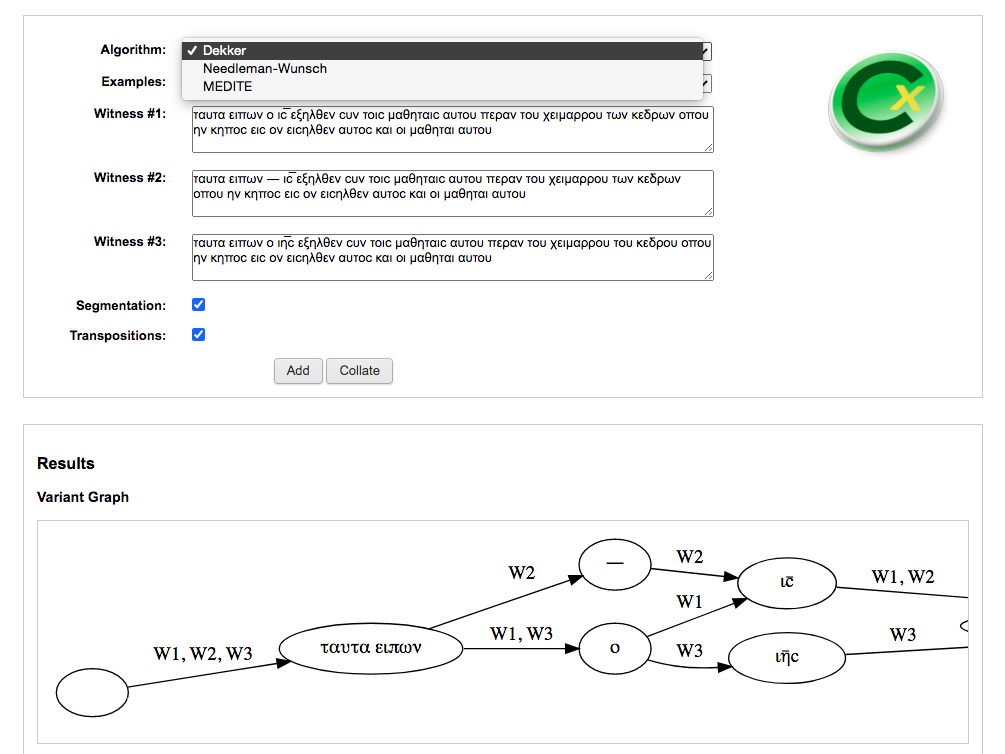
\includegraphics[width=.95\textwidth]{imgs/collatex.png}
	\end{center}
\end{frame}

\begin{frame}
    \frametitle{Strumenti per edizioni critiche}
    \framesubtitle{Strumenti di collazione automatica}
	\addtocounter{nframe}{1}
    \begin{center}
        \textbf{Variance Viewer}
    \end{center}
    \begin{center}
        \textit{\url{http://variance-viewer.informatik.uni-wuerzburg.de/Variance-Viewer/}}
	\end{center}
    \begin{center}
        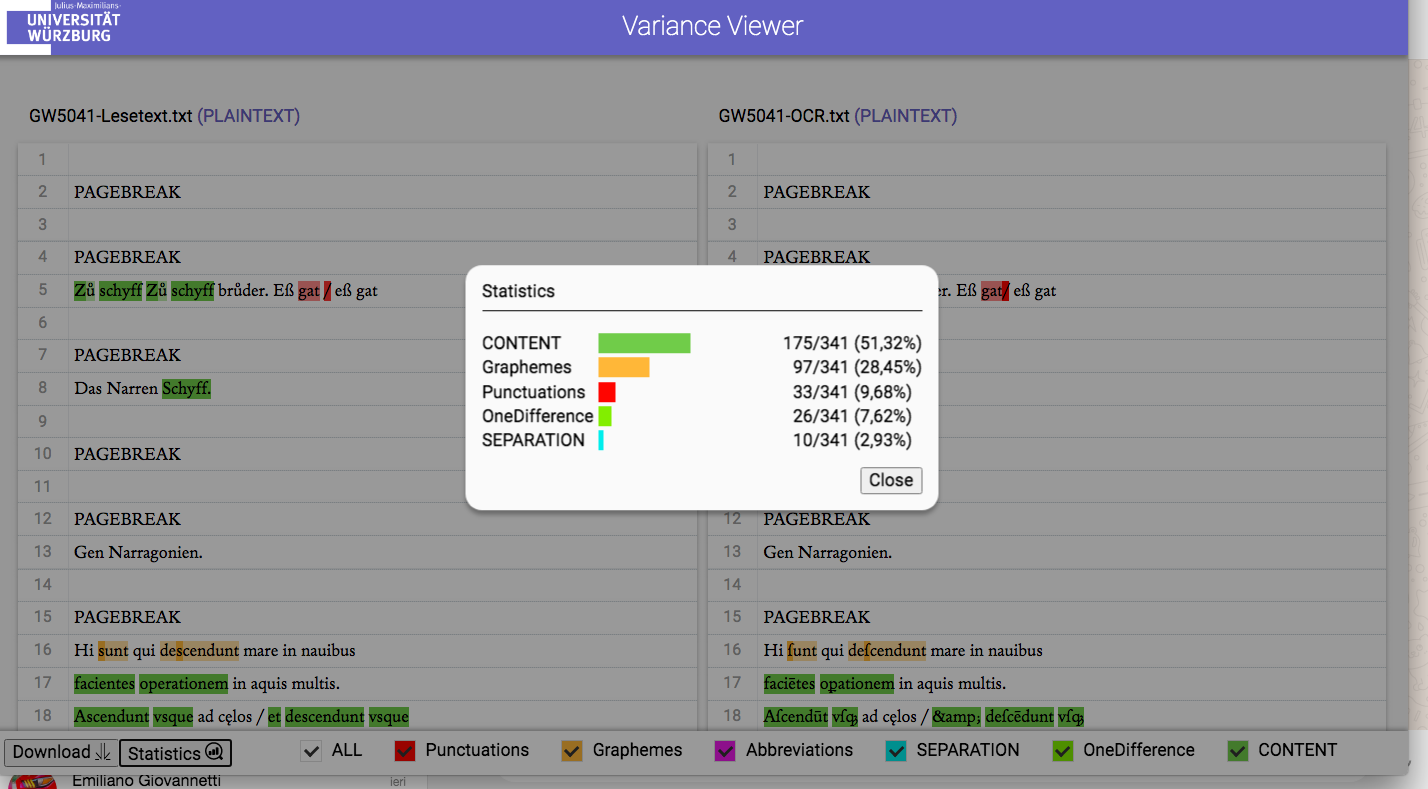
\includegraphics[width=.95\textwidth]{imgs/variance-viewer.png}
	\end{center}
\end{frame}

\begin{frame}
    \frametitle{Strumenti per edizioni critiche}
    \framesubtitle{Strumenti di collazione automatica}
	\addtocounter{nframe}{1}
    \begin{center}
        \textbf{Juxta Web Service}
    \end{center}
    \begin{center}
        \textit{\url{http://juxtacommons.org/}}
	\end{center}
    \begin{center}
        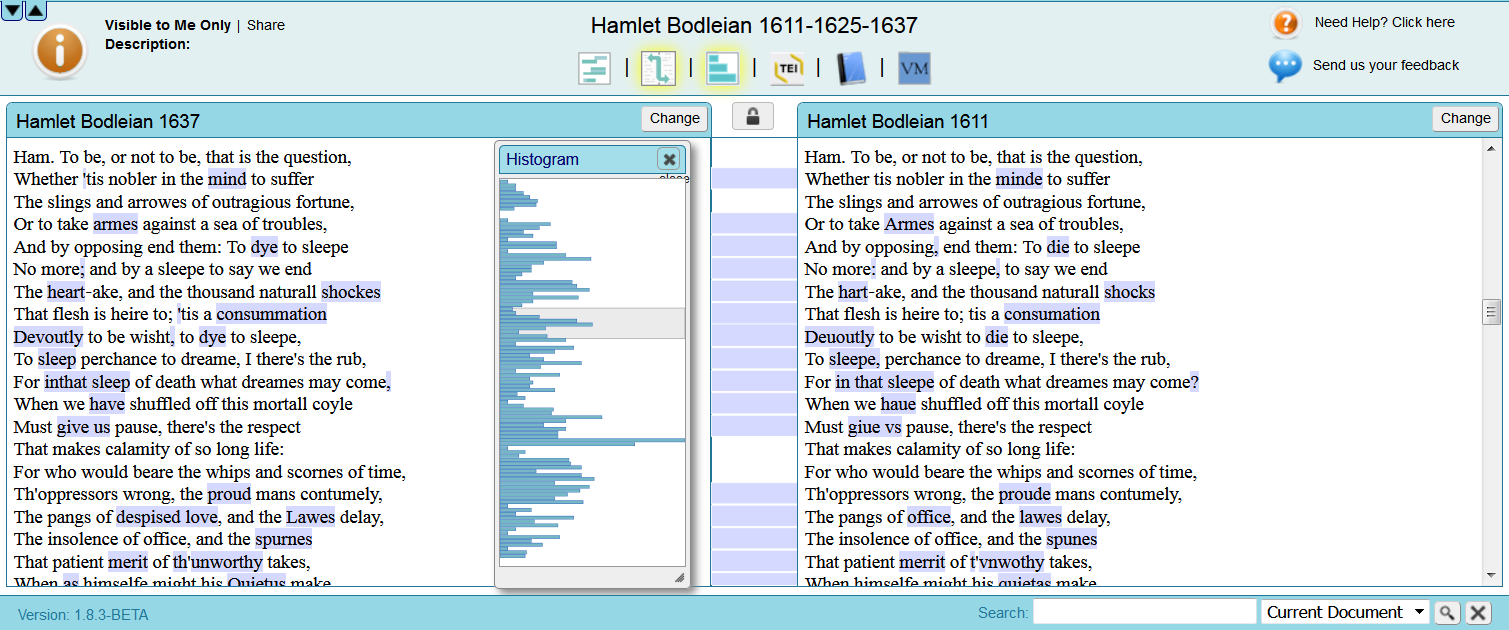
\includegraphics[width=.95\textwidth]{imgs/juxtaweb.png}
	\end{center}
\end{frame}

\begin{frame}
    \frametitle{Strumenti per edizioni critiche}
    \framesubtitle{Strumenti di collazione automatica}
	\addtocounter{nframe}{1}
    \begin{center}
        \textbf{StemmaWeb}
    \end{center}
    \begin{center}
        \textit{\url{https://stemmaweb.net/stemmaweb/}}
	\end{center}
    \begin{center}
        \includegraphics[width=.95\textwidth]{imgs/}
	\end{center}
\end{frame}

\begin{frame}
    \frametitle{Strumenti per edizioni critiche}
    \framesubtitle{Strumenti di collazione automatica}
	\addtocounter{nframe}{1}
    \begin{center}
        \textbf{TUebingen System of Text Processing Programs" TUSTEP - TXSTEP}
    \end{center}
    \begin{center}
        \textit{\url{https://www.tustep.uni-tuebingen.de/tustep_eng.html}}
	\end{center}
    \begin{center}
        %\includegraphics[width=.95\textwidth]{imgs/}
        TODO
	\end{center}
\end{frame}

\begin{frame}
    \frametitle{Strumenti per edizioni critiche}
    \framesubtitle{Strumenti di collazione automatica}
	\addtocounter{nframe}{1}
    \begin{center}
        \textbf{MEDITE}
    \end{center}
    \begin{center}
        \textit{\url{http://www-poleia.lip6.fr/~ganascia/Medite_Project}}
	\end{center}
    \begin{center}
        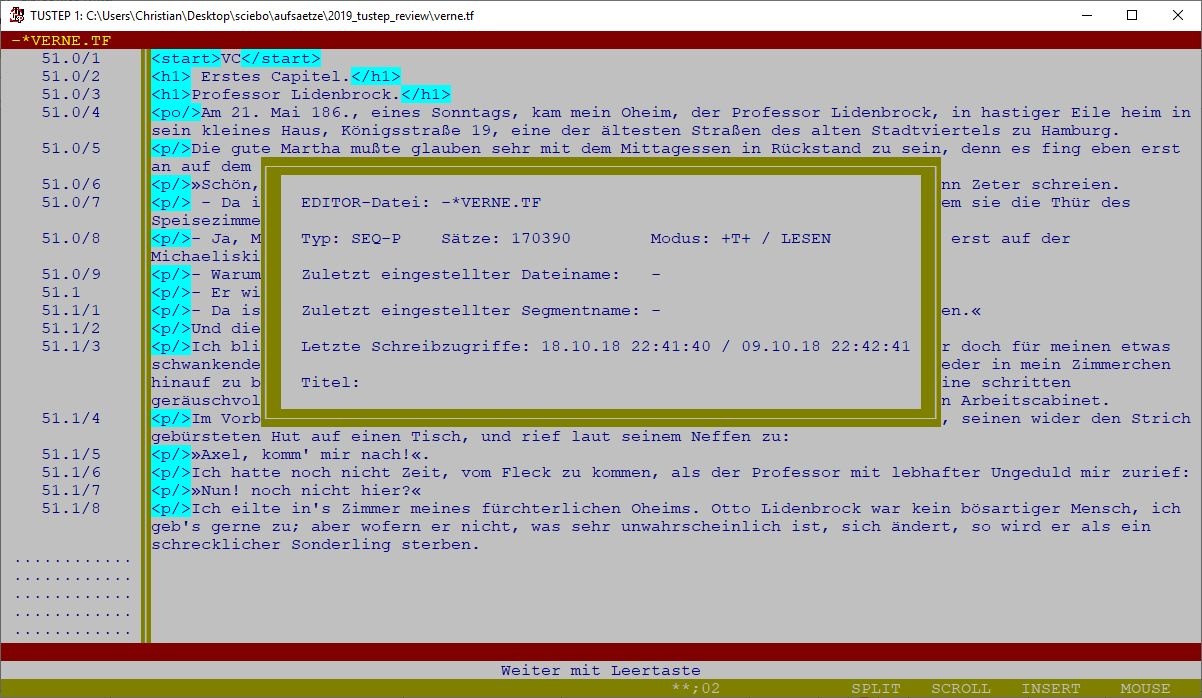
\includegraphics[width=.95\textwidth]{imgs/tustep.jpg}
	\end{center}
\end{frame}




\begin{frame}
    \frametitle{Strumenti per edizioni critiche}
    \framesubtitle{Strumenti per la visualizzazione e pubblicazione}
	\addtocounter{nframe}{1}
    \begin{center}
        \textbf{Classical Text Editor}
    \end{center}
    \begin{center}
        \textit{\url{https://cte.oeaw.ac.at/}}
	\end{center}
    \begin{center}
        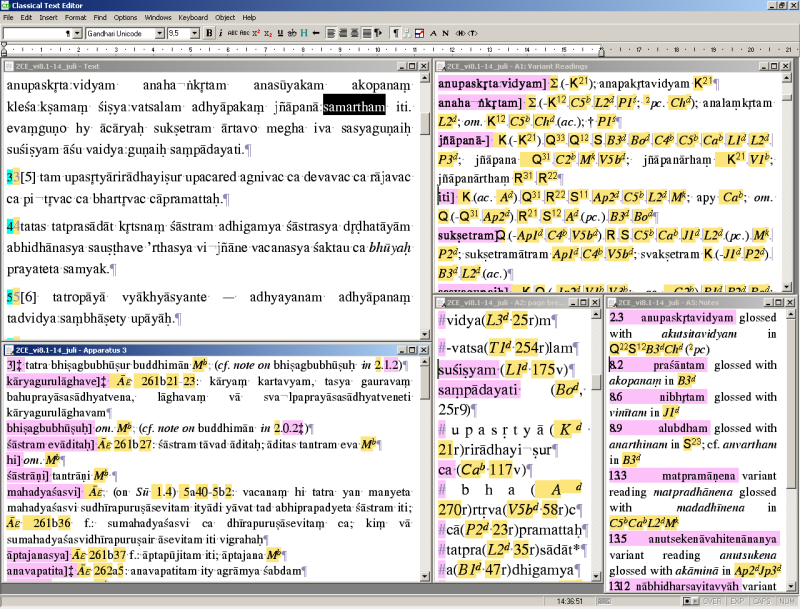
\includegraphics[width=.95\textwidth]{imgs/cte.gif}
	\end{center}
\end{frame}

\begin{frame}
    \frametitle{Strumenti per edizioni critiche}
    \framesubtitle{Strumenti per la visualizzazione e pubblicazione}
	\addtocounter{nframe}{1}
    \begin{center}
        \textbf{TEIpublisher}
    \end{center}
    \begin{center}
        \textit{\url{https://teipublisher.com/index.html}}
	\end{center}
    \begin{center}
        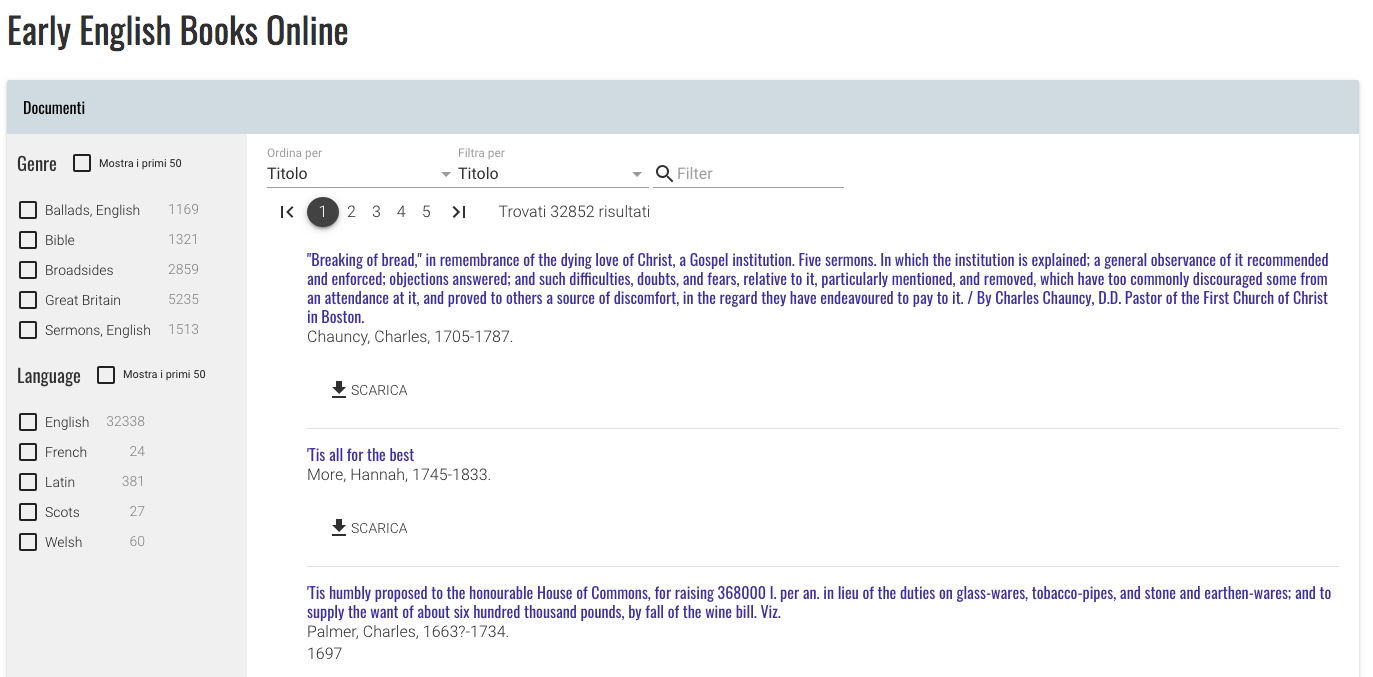
\includegraphics[width=.95\textwidth]{imgs/teipublisher.png}
	\end{center}
\end{frame}

\begin{frame}
    \frametitle{Strumenti per edizioni critiche}
    \framesubtitle{Strumenti per la visualizzazione e pubblicazione}
	\addtocounter{nframe}{1}
    \begin{center}
        \textbf{Edition Visualization Technology (EVT)}
    \end{center}
    \begin{center}
        \textit{\url{http://evt.labcd.unipi.it}}
	\end{center}
    \begin{center}
        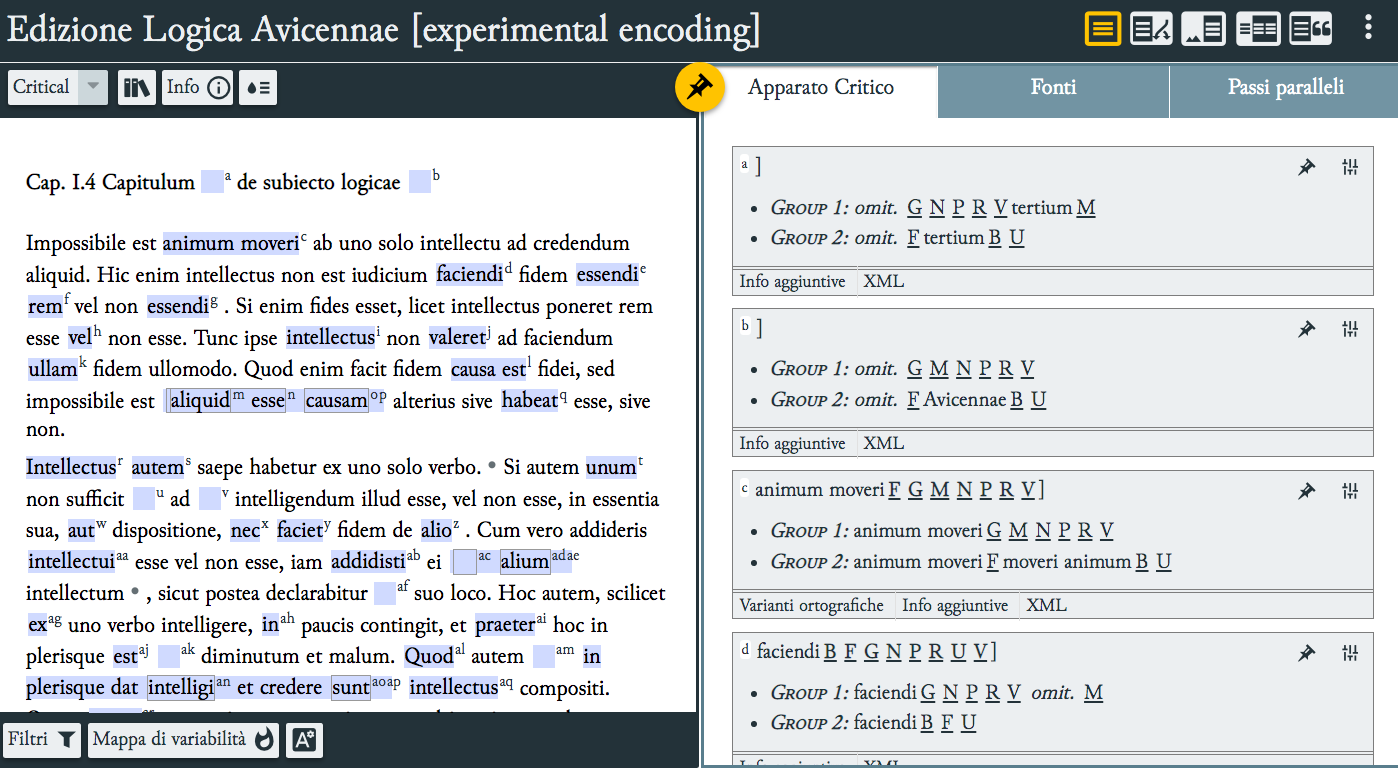
\includegraphics[width=.95\textwidth]{imgs/evt.png}
	\end{center}
\end{frame}

\begin{frame}
    \frametitle{Strumenti per edizioni critiche}
    \framesubtitle{Strumenti per la visualizzazione e pubblicazione}
	\addtocounter{nframe}{1}
    \begin{center}
        \textbf{Textual Communities}
    \end{center}
    \begin{center}
        \textit{\url{https://textualcommunities.org/app/}}
	\end{center}
    \begin{center}
        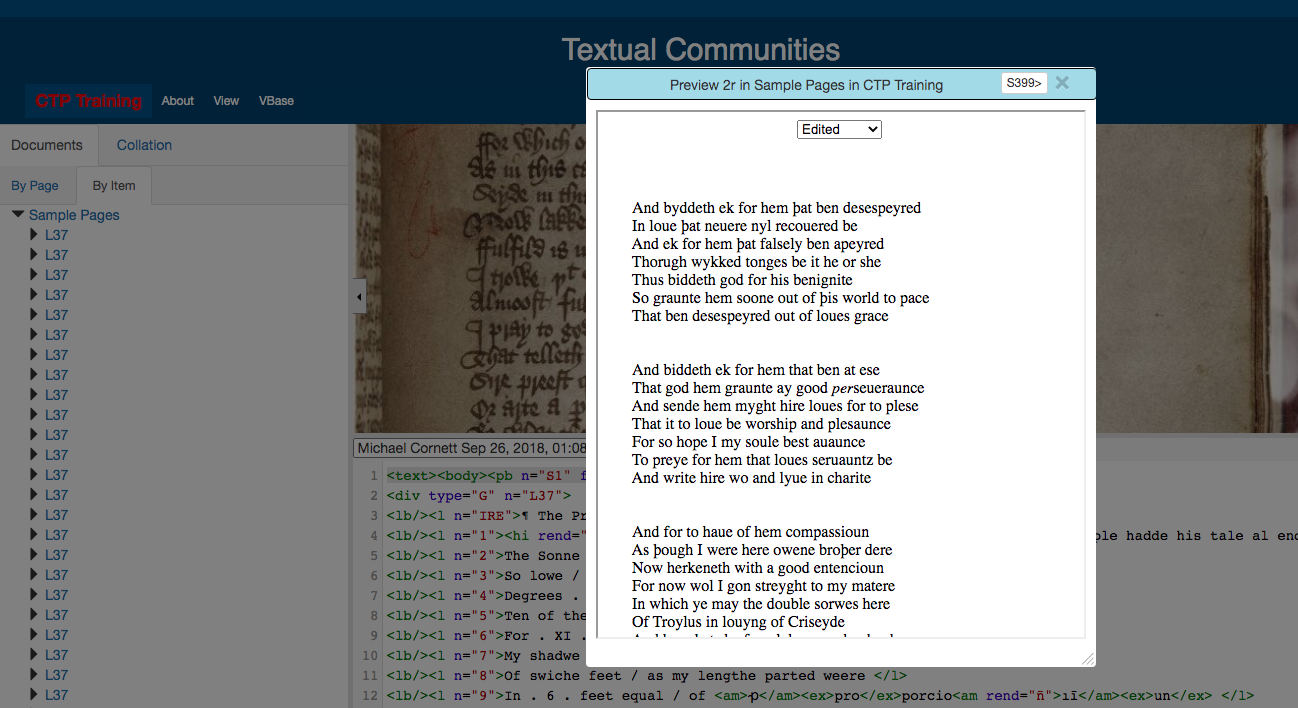
\includegraphics[width=.95\textwidth]{imgs/textualcommunities.png}
        
	\end{center}
\end{frame}

\begin{frame}
    \frametitle{Strumenti per edizioni critiche}
    \framesubtitle{Strumenti per la visualizzazione e pubblicazione}
	\addtocounter{nframe}{1}
    \begin{center}
        \textbf{Versioning Machine}
    \end{center}
    \begin{center}
        \textit{\url{http://v-machine.org}}
	\end{center}
    \begin{center}
        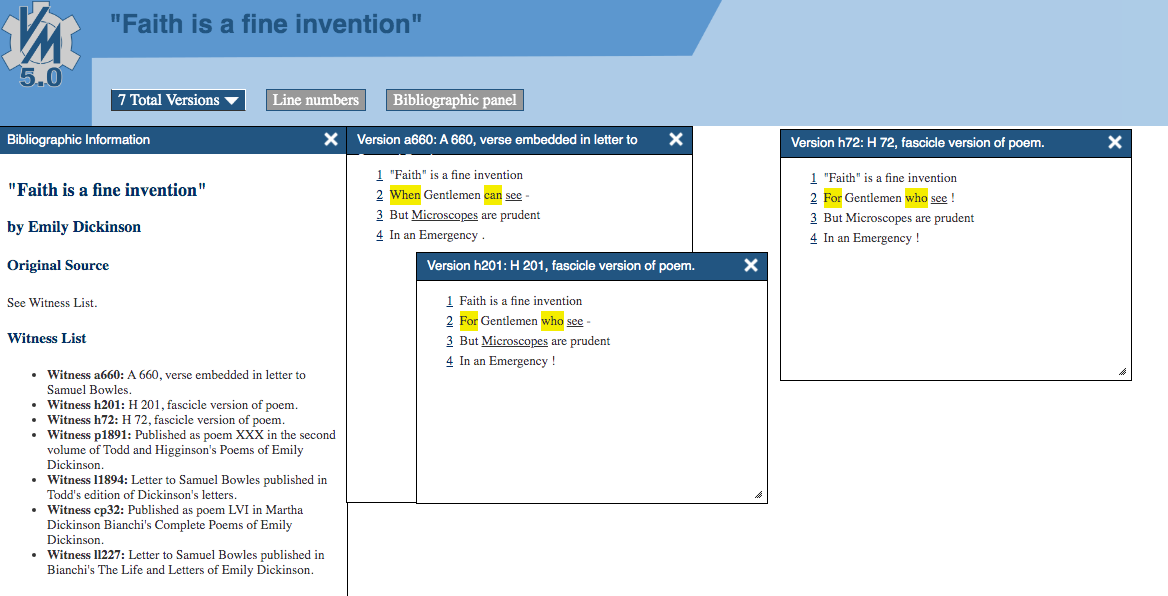
\includegraphics[width=.95\textwidth]{imgs/v-machine.png}
	\end{center}
\end{frame}

\begin{frame}
    \frametitle{Strumenti per edizioni critiche}
    \framesubtitle{Strumenti per la visualizzazione e pubblicazione}
	\addtocounter{nframe}{1}
    \begin{center}
        \textbf{LERA/SADA project}
    \end{center}
    \begin{center}
        \textit{\url{https://sada.uzi.uni-halle.de/}}
	\end{center}
    \begin{center}
        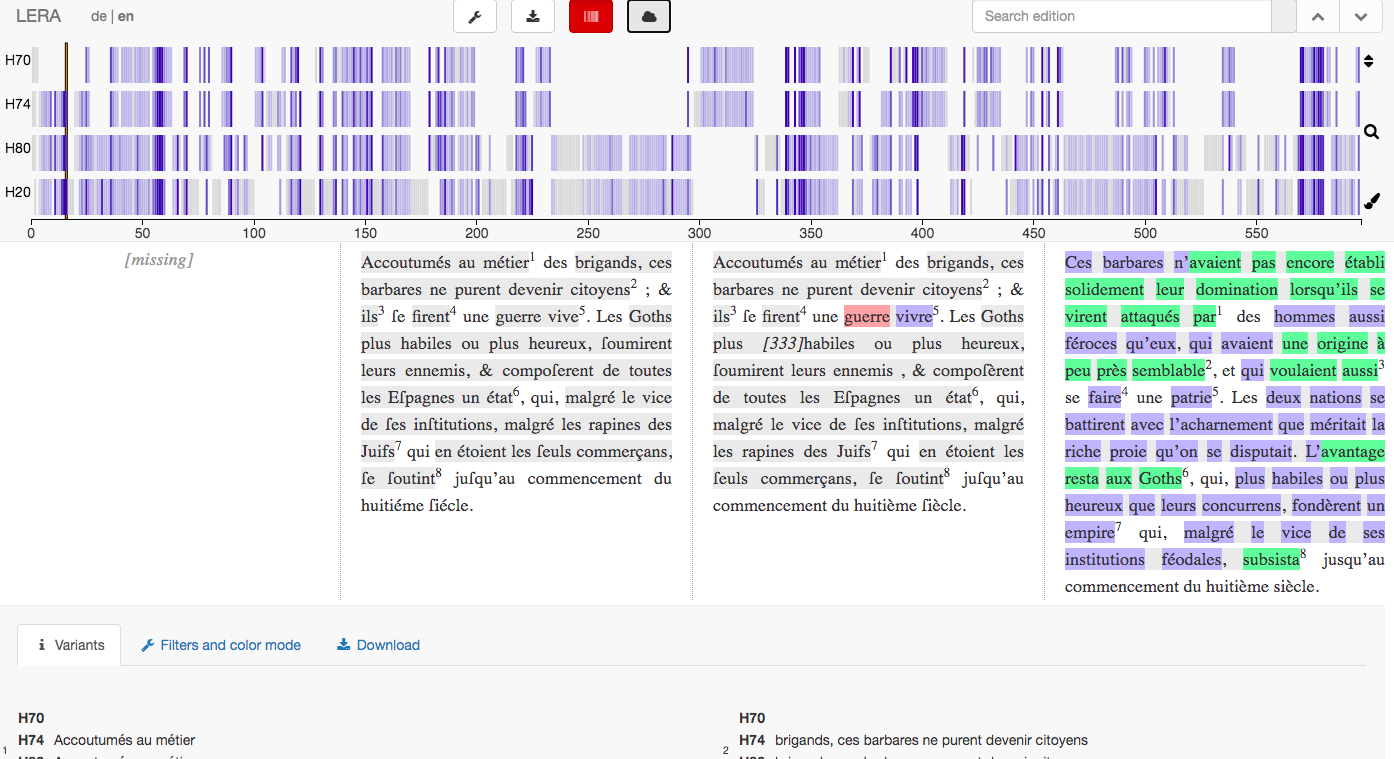
\includegraphics[width=.95\textwidth]{imgs/lara.png}
	\end{center}
\end{frame}

\begin{frame}
    \frametitle{Strumenti per edizioni critiche}
    \framesubtitle{Strumenti per la visualizzazione e pubblicazione}
	\addtocounter{nframe}{1}
    \begin{center}
        \textbf{Critical Edition Toolbox}
    \end{center}
    \begin{center}
        \textit{\url{http://teicat.huma-num.fr/index.php}}
	\end{center}
    \begin{center}
        \includegraphics[width=.95\textwidth]{imgs/}
	\end{center}
\end{frame}

\begin{frame}
    \frametitle{Strumenti per edizioni critiche}
    \framesubtitle{Strumenti per la visualizzazione e pubblicazione}
	\addtocounter{nframe}{1}
    \begin{center}
        \textbf{LaTex/Reledmac}
    \end{center}
    \begin{center}
        \textit{\url{https://ctan.org/pkg/reledmac}}
	\end{center}
    \begin{center}
        \includegraphics[width=.95\textwidth]{imgs/}
	\end{center}
\end{frame}

\begin{frame}
    \frametitle{Strumenti per edizioni critiche}
    \framesubtitle{Strumenti per la visualizzazione e pubblicazione}
	\addtocounter{nframe}{1}
    \begin{center}
        \textbf{TRAVIZ/ITEAL}
    \end{center}
    \begin{center}
        \textit{\url{http://www.traviz.vizcovery.org/}}
	\end{center}
    \begin{center}
        \includegraphics[width=.95\textwidth]{imgs/}
	\end{center}
\end{frame}

\begin{frame}
    \frametitle{Strumenti per edizioni critiche}
    \framesubtitle{Strumenti per la visualizzazione e pubblicazione}
	\addtocounter{nframe}{1}
    \begin{center}
        \textbf{EUPORIA}
    \end{center}
    \begin{center}
        \textit{cophilab.ilc.cnr.it}
	\end{center}
    \begin{center}
        \includegraphics[width=.95\textwidth]{imgs/}
	\end{center}
\end{frame}
